\documentclass[12pt,fleqn]{article}
\usepackage[margin=1in,top=1in,bottom=1in]{geometry}
\usepackage{mathtools}
\usepackage{longtable}
\usepackage{enumitem}
\usepackage{hyperref}
\usepackage[dvips]{graphics}
\usepackage[table]{xcolor}
\usepackage{amssymb}
\usepackage{subfig}
\usepackage{booktabs}
\usepackage{tikz}
\usepackage{pdflscape}

\usepackage[normalem]{ulem}

\usepackage{multicol}
\usepackage{txfonts}
%\usepackage{amsfonts}
\usepackage{natbib}

\usepackage{gb4e}
%\usepackage{/Users/judith/Library/Latex/drs}
%\usepackage{/Users/judith/Library/Latex/avm}
\usepackage[all]{xy}
\usepackage{rotating}
\usepackage{tipa}
\usepackage{multirow}
\usepackage{authblk}
\usepackage{adjustbox}
\usepackage{array}

\usepackage{titlesec}
\titleformat*{\section}{\bfseries\footnotesize}
 
\setlength{\parindent}{0cm}
\setlength{\parskip}{0ex}

\setlength{\bibsep}{0mm}
\bibpunct[:]{(}{)}{;}{a}{,}{,}


\newcommand{\yi}{\'{\symbol{16}}}
\newcommand{\nasi}{\~{\symbol{16}}}
\newcommand{\hina}{h\nasi na}
\newcommand{\ina}{\nasi na}


\setlength{\bibhang}{0.5in}
\setlength{\bibsep}{0mm}
\bibpunct[:]{(}{)}{,}{a}{}{,}

\newcommand{\6}{\mbox{$[\hspace*{-.6mm}[$}} 
\newcommand{\9}{\mbox{$]\hspace*{-.6mm}]$}}
\newcommand{\sem}[2]{\6#1\9$^{#2}$}
\renewcommand{\ni}{\~{\i}}

 \begin{document}
 
%The main text should be at most 2 pages (US Letter or A4) in length, including examples, with an optional 3rd page for references or also large graphs, tables, pictures and figures.
 
\begin{center}
{\large \bf Prior probabilities and the projectivity of entailed and non-entailed content}
\end{center}

This paper provides experimental evidence from English utterances with clause-embedding predicates that i) the content of both entailed and non-entailed clausal complements may be projective, ii) the projectivity of entailed and non-entailed content is influenced by the prior probability of the event described by the clause, and iii) veridicality (a gradient measure of the extent to which the clausal complement is entailed) is not a predictor of projectivity. These findings challenge analyses of projective content that are limited to entailed content (e.g., \citealt{heim83,vds92}) and motivate analyses according to which listeners integrate multiple sources of information, some conventional and some non-conventional, in determining what speakers are committed to (e.g., \citealt{brst-salt10,brst-ar,abrusan2011,abrusan2016,tbd-variability}). 

{\bf Presuppositions versus non-entailed projective content} 

The content of the clausal complement in (\ref{embedded}), that Julian dances salsa, is `projective': a speaker who utters one of the variants in (\ref{embedded}) may be taken to be committed to this content even though the clause occurs in a polar question (e.g., \citealt{ccmg90}). The question of how this content comes to be projective is traditionally given very different answers for {\em discover} vs.\ {\em announce}. Whereas the content of the complement of {\em discover} is typically taken to be projective because it is a presupposition (e.g., \citealt{heim83,vds92}), the content of the complement of {\em announce} is not analyzed as a presupposition because it is not entailed by the atomic sentence in (\ref{unembedded}), in contrast to the content of the complement of {\em discover}. Thus, whereas {\em discover} is considered to be a factive predicate (i.e., it both entails and presupposes the content of its complement), {\em announce} is merely a ``part-time trigger'' (\citealt[139]{schlenker10}) that gives rise to the ``illusion of factivity'' (\citealt[76]{anand-hacquard2014}).

\vspace*{-.2cm}
\begin{exe}
\ex
\begin{xlist}
\ex\label{embedded} Did Sandy \{discover / announce\} that Julian dances salsa?
\ex\label{unembedded} Sandy \{discovered / announced\} that Julian dances salsa.
\end{xlist}
\end{exe}
\vspace*{-.2cm}

This paper provides experimental evidence that suggests that it is empirically inadequate to analyze the projectivity of entailed and non-entailed content in fundamentally different ways. 

{\bf Factors that influence the projectivity of projective content}

The projectivity of (entailed) projective content is variable (e.g., \citealt{karttunen71b,kadmon01,tbd-variability}) and influenced by several conventional and non-conventional factors, incl.\ syntax (e.g., \citealt{potts05}), context (e.g., \citealt{beaver-belly}), prosody (e.g., \citealt{cummins-rohde2015,tonhauser-salt26}) and at-issueness (e.g., \citealt{tbd-variability}). We examined the influence of two novel factors on the projectivity of the content of the clausal complements: the prior probability of the event described by the clausal complement and the veridicality of the clause-embedding predicate. English-speaking participants were recruited on Amazon's Mechanical Turk platform.

\vspace*{.7ex}

\underline{Norming study \#1 (n=95):} We measured the prior probabilities of 20 events described by English clauses (e.g., {\em Julian dances salsa}) given one of two facts about the world for each event: one fact made the event more likely than the other fact (e.g., {\em Julian is Cuban} vs.\ {\em Julian is German}). The mean prior probability of the events was .7 (sd = .21) when presented with facts that made the events more likely and .16 (sd = .17) when presented with facts that make the events less likely.

\vspace*{.7ex}

\underline{Norming study \#2 (n=300):} Veridicality was defined as the extent to which sentences like (\ref{stim-veri}) were judged to be contradictory (e.g., for (\ref{stim-veri}): Is Carol's utterance contradictory?). Responses were given on a sliding scale from `definitely no' to `definitely yes'. 
\vspace*{-.2cm}
\begin{exe}
\ex\label{stim-veri} {\bf Carol:} Sandra \{discovered / announced / suggested\} that Julian dances salsa, but he doesn't. 
\end{exe}
\vspace*{-.2cm}
The veridicality of 20 clause-embedding predicates was tested: 7 are typically taken to entail the content of the complement (E: {\em be annoyed, know, discover, reveal, see, establish, be right}), 5 are typically taken to not entail the content of the complement (NE: {\em pretend, think, suggest, say, hear}), and the remaining 8 are typically taken to not entail the content of the complement even though they may sometimes appear to (V: {\em prove, demonstrate, confess, inform, announce, acknowledge, admit, confirm}); see e.g., \citealt{schlenker10,swanson2012,anand-hacquard2014}. Each predicate was paired with the 20 clauses that describe the aforementioned events. As shown in Fig.~\ref{f-veridicality}, predicates in the NE class are least veridical, as expected, but predicates in the E class are not uniformly highly veridical and instead form a veridicality gradient with predicates in the V class.

{\bf Experiment: Projectivity}

This experiment explored the influence of prior probability and veridicality on the projectivity of the contents of clausal complements. Of the 20 predicates, 6 are typically taken to be factive ({\em be annoyed, know, discover, reveal, see, hear}), 7 are typically taken to not be factive ({\em be right, pretend, think, suggest, say, prove, demonstrate}), and the remaining 7 predicates have been suggested to be ``part-time triggers'' or to give rise to the ``illusion of factivity'' ({\em establish,  confess, announce, acknowledge, admit, confirm, inform}); see references above.

\underline{Materials and procedure.} 400 polar questions were formed from the 20 predicates paired with the 20 event-describing complement clauses. Participants were presented with 20 polar questions (one for each predicate), uttered by a named speaker, as shown in (\ref{stim-project}). Each polar question was presented with one of the two facts for the event described by clausal complement. Participants were asked to assess whether the speaker is certain of the content of the clausal complement (e.g., \emph{Is Carol certain that Julian dances salsa?}) and gave their responses on a sliding scale from `no' to `yes'. 
\vspace*{-.2cm}
\begin{exe}
\ex\label{stim-project} {\bf Fact (which Carol knows):} Julian is German.  \\ 
{\bf Carol:} Did Sandra \{discover / announce / suggest\} that Julian dances salsa?
\end{exe}
\vspace*{-.2cm}

\underline{Results (n=300).}  Mean projectivity ratings are shown in Fig.~\ref{f-projectivity}. Replicating \citealt{tbd-variability}, we observe a large degree of variability in projectivity across predicates. The contents of clausal complements that describe a priori more likely events were judged to be more projective than those that described a priori less likely events ($\beta$ = .34, $SE$ = .03, $t$ = 10.6, $p <$ .0001), as revealed by a mixed effects linear regression predicting projectivity rating from fixed effects of mean prior probability (from norming study \#1), mean veridicality rating (from norming study \#2), and their interaction, as well as from random effects for participant, verb, clausal complement, and fact. Neither the main effect of veridicality nor its interaction with prior reached significance ($p >$ .26). This was true whether the analysis was conducted on the full dataset or only on projective contents (contents of complements of {\em announce} and predicates to its right in  Fig.~\ref{f-projectivity}).

{\bf Discussion and theoretical implications}

Although projectivity is obviously influenced by the lexical meaning of clause-embedding predicates (e.g., \citealt{karttunen71b,tbd-variability}), our findings do not support the assumption that entailment determines the empirical purview of analyses of projection. For instance, even though the veridicality of {\em reveal, be annoyed} and {\em confess} is statistically indistinguishable, the content of the complement of {\em be annoyed} is significantly more projective than that of {\em reveal} or {\em confess}. Our findings are instead compatible with analyses of projection that are not restricted to entailed content and according to which listeners integrate multiple sources of information, including prior event probabilities, in determining what speakers are committed to (see references above). Which lexical meaning properties of predicates influence projectivity is a pressing question for future research. 
 

%\newpage
%
%\begin{itemize}
%
%\item {\em establish, confirm} did not come out as projective, contrary to assumptions (confirm: ``illusion of factivity'') and previous findings (establish, variability paper)
%
%\item factive {\em be annoyed, know, inform, see, hear, discover} are 6 most projective predicates, but {\em be annoyed, inform, hear} were significantly less veridical than {\em know, see} 
%
%{\em inform, announce} did not differ in veridicality (.5, lots of variability), but {\em inform} significantly more projective than {\em announce} 
%
%\item {\em acknowledge, admit}: ``illusion of factivity'', but 7th and 8th most projective, 
%
%{\em acknowledge} indistinguishable from factive {\em reveal, hear, discover, see}
%
%{\em admit} indistinguishable from factive {\em discover, hear, reveal}
%
%\item factive {\em reveal} (9th highest) indistinguishable from `illusion'' {\em acknowledge, admit, announce, confess, demonstrate, establish}
%
%\item `illusion'' {\em confess} (10th highest) indistinguishable from factive {\em reveal}, marginally different from {\em discover}
%
%\item {\em announce} is the lowest clearly projective predicate: mean of factH above .5 and significantly different from {\em think}
%
%
%
%\end{itemize}

\newpage

\begin{figure}[h!]
\centering

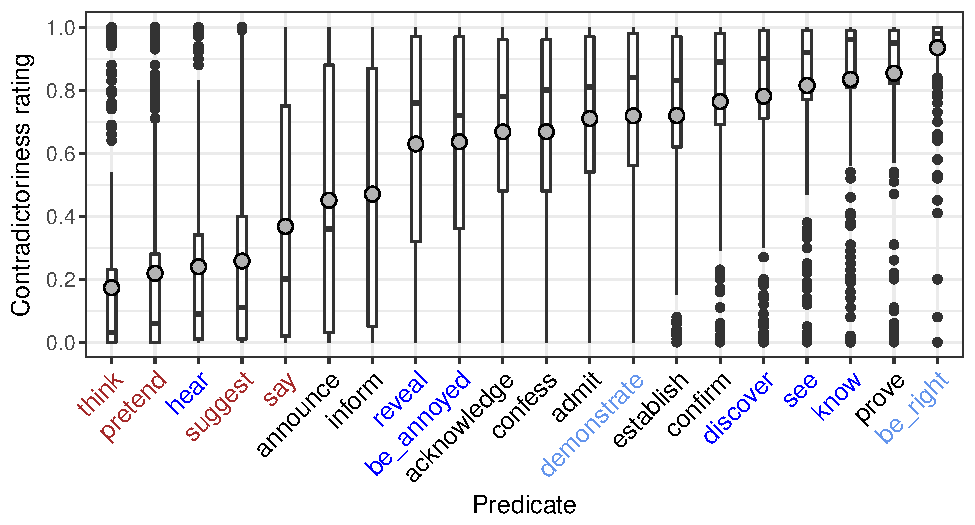
\includegraphics[width=.46\paperwidth]{../results/2-veridicality2/graphs/boxplot-veridicality}

\caption{\footnotesize{Boxplot of contradictoriness (veridicality) ratings by predicate, collapsing across complements. Grey dots indicate means and notches indicate medians. Colors code veridicality classes E (blue), NE (brown) and V (green).}}
\label{f-veridicality}
\end{figure}

\vspace*{-.8cm}

\begin{figure}[h!]
\centering

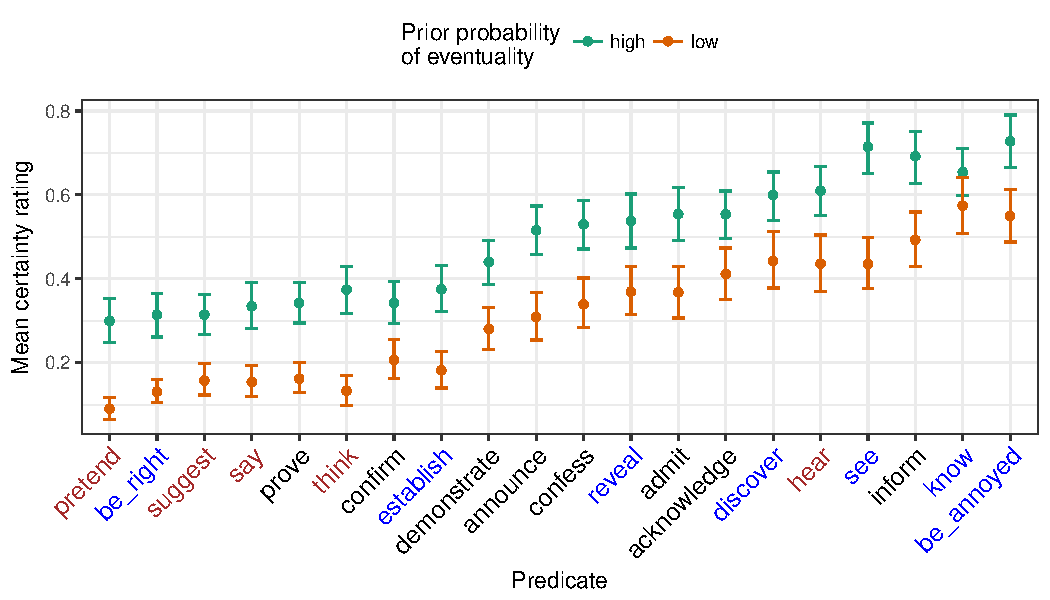
\includegraphics[width=.6\paperwidth]{../results/3-projectivity/graphs/means-projectivity-by-predicate-and-facttype}

\caption{\footnotesize{Mean certainty (projectivity) ratings by predicate and fact type, collapsing across complements. Error bars indicate 95\% confidence intervals. Colors code veridicality classes E (blue), NE (brown) and V (green).}}
\label{f-projectivity}
\end{figure}

\vspace*{-1cm}

\begin{scriptsize}
\bibliographystyle{/Users/tonhauser.1/Library/Latex/cslipubs-natbib}
\bibliography{../bibliography}
\end{scriptsize}

\end{document}
